\documentclass[pdflatex,compress]{beamer}

%\usetheme[dark,framenumber,totalframenumber]{ElektroITK}
\usetheme[darktitle,framenumber,totalframenumber]{ElektroITK}

\usepackage{graphicx}

\title{METODE NUMERIK}
\subtitle{Pengantar Metode Numerik}

\author{Tim Dosen Pengampu}

\begin{document}

% ----------------------------------------------------------------------------
% *** Titlepage <<<
% ----------------------------------------------------------------------------
\maketitle
% ----------------------------------------------------------------------------
% *** END of Titlepage >>>
% ----------------------------------------------------------------------------

% ----------------------------------------------------------------------------
\section{Kontrak Perkuliahan}

\begin{frame}
\frametitle{Kontrak Perkuliahan}
	\begin{enumerate}
		\item Bahan kajian, bobot evaluasi, dll $\rightarrow$ Baca RPS.
	\end{enumerate}
\end{frame}

% ----------------------------------------------------------------------------
\section{Pengantar Metode Numerik}

\begin{frame}
\frametitle{Apa itu Metode Numerik?}
	\begin{itemize}
		\item \textbf{Numerik:} berhubungan dengan angka.
		\item \textbf{Metode:} cara yang sistematis untuk menyelesaikan persoalan guna mencapai tujuan yang ditentukan.
		\item \textbf{Metode Numerik:} cara sistematis untuk menyelesaikan persoalan matematika dengan operasi angka (+, -, *, /).
	\end{itemize}
\end{frame}

\begin{frame}
\frametitle{Contoh persoalan matematika}
	\begin{enumerate}
		\item Tentukan akar-akar persamaan polinom:
		\[ 23.4x^7 - 1.25x^6 + 120x^4 + 15x^3 - 120x^2- x + 100 = 0
		 \]
		 \item Tentukan nilai $ x $ yang memenuhi persamaan:
		 \[ \sqrt{27.8e^{5x} - \frac{1}{x}} = \cos^{-1}\frac{(120x^2 + \sqrt{2x})}{17x-65}\]
		 \item Hitung nilai integral-tentu berikut:
		 \[ \int_{1.2}^{2.5} \left( \sqrt{\left(45.3e^{7x}+\frac{100}{x}\right)^4} + \frac{4}{(x^2 + 1)} \right) dx \]
	\end{enumerate}
\end{frame}

\begin{frame}
	\begin{enumerate}
		\setcounter{enumi}{3}
		\item Diberikan persamaan differensial biasa (PDB) dengan sebuah nilai awal:
		\[ 150y'' + 2y't = \frac{\sqrt{\ln(21t+40)y}}{t^2} + 120;~y(0)=1 \]
		Hitung nilai $ y $ pada saat $ t = 1.8 $
	\end{enumerate}
\end{frame}

\begin{frame}
	\begin{enumerate}
		\setcounter{enumi}{4}
		\item Selesaikan sistem persamaaan linear:
		\begin{align*}
			1.2a - 3b -  12c + 12d + 4.8e - 5.5f	+ 100g  &= 18 \\
			0.9a + 3b -    c + 16d +   8e -   5f	-  10g  &= 17 \\
			4.6a + 3b -   6c -  2d +   4e + 6.5f	-  13g  &= 19 \\
			3.7a - 3b +   8c -  7d +  14e + 8.4f	+  16g  &=  6 \\
			2.2a + 3b +  17c +  6d +  12e - 7.5f	+  18g  &=  9 \\
			5.9a + 3b +  11c +  9d -   5e -  25f	-  10g  &=  0 \\
			1.6a + 3b + 1.8c + 12d -   7e + 2.5f	+    g  &= -5
		\end{align*}
	\end{enumerate}
\end{frame}

\begin{frame}
\frametitle{Cara penyelesaian \\
	persoalan matematika}
	\begin{itemize}
		\item Cara penyelesaian persoalan matematika ada 2:
		\begin{enumerate}
			\item \textbf{Secara analitik:} menggunakan rumus dan teoremayang sudah baku di dalam matematika $\rightarrow$ metode analitik.
			\item \textbf{Secara numerik:} menggunakan pendekatan aproksimasi untuk mencari solusi hanya dengan operasi aritmatika biasa $\rightarrow$ metode numerik.
		\end{enumerate}
	\end{itemize}
\end{frame}

\begin{frame}
	\frametitle{Contoh 1}
	$ x^2 - 6x + 8 = 0 \rightarrow $ Carilah akar-akarnya! \\
	\begin{enumerate}
		\item Metode analitik: faktorkan menjadi $$ (x-4)(x-2) = 0 $$
			\begin{align*}
				x - 4 = 0 &\rightarrow x_1 = 4 \\
				x - 2 = 0 &\rightarrow x_2 = 2
			\end{align*}
	\end{enumerate}
\end{frame}

\begin{frame}
	\begin{enumerate}
		\setcounter{enumi}{1}
		\item Metode Numerik: Diketahui sebuah akar terletak di dalam selang [3, 6] $\rightarrow$ mengapa?
			
			\begin{figure}
				\centering
				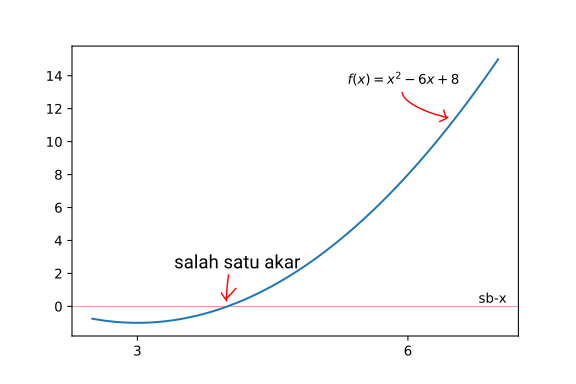
\includegraphics[width=0.8\linewidth]{img/img001}
				\label{fig:img001}
			\end{figure}
				
	\end{enumerate}
\end{frame}

\begin{frame}
	Pendekatan sederhana mencari akar adalah secara iteratif dengan \textbf{metode titik tengah} (\textit{bisection method})
	
	\begin{enumerate}
		\item bagi selang $ [a,b] $ menjadi dua dengan titik tengah, $ c = (a + b) / 2 $
		\item ada dua sub-selang: $ [a, c] $ dan $ [c, b] $. Pilih selang iterasi yang baru dengan syarat nilai fungsi di ujung selang berbeda tanda.
		\item ulangi langkah 1 dan 2 sampai ukuran selang $ < \varepsilon$ (epsilon adalah nilai yang sangat kecil yang menyatakan toleransi kesalahan akar yang diinginkan, misalnya $\varepsilon$ = 0.001, 000001, dsb
	\end{enumerate}
\end{frame}

\begin{frame}
	\begin{center}
		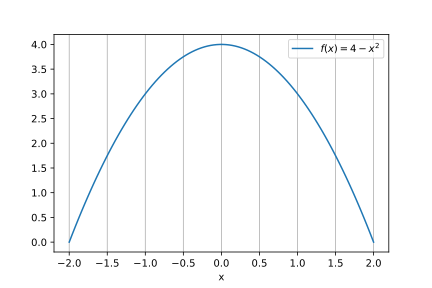
\includegraphics[width=\linewidth]{img/img002}
	\end{center}
\end{frame}

\begin{frame}
	\begin{itemize}
		\item Mencari akar $ f(x) = x^2 - 6x + 8 = 0 $ di dalam selang $ [3, 6] $ dengan $ \varepsilon = 0.0005 $
		
		\begin{center}
			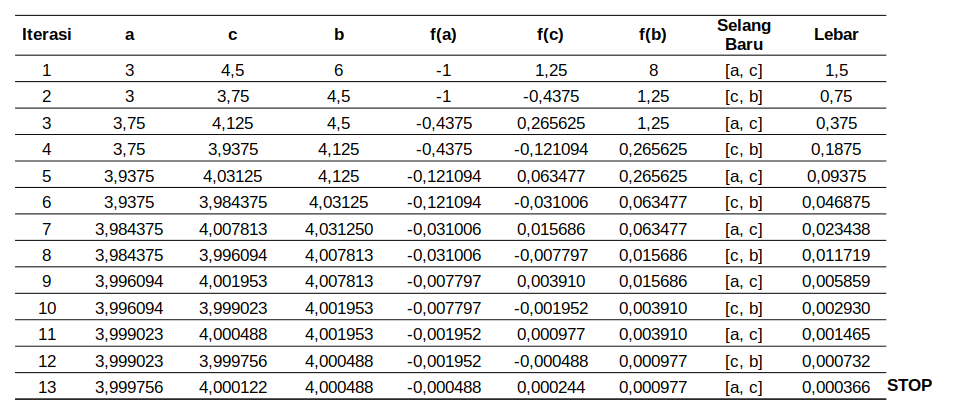
\includegraphics[width=\linewidth]{img/tab001}
		\end{center}
	
		\item Aproksimasi akar = 4.000122
	\end{itemize}
\end{frame}

\begin{frame}
	\frametitle{Contoh 2}

	Hitung integral $ \int_{-1}^{1} (4 - x^2) dx $
	
	\begin{enumerate}
		\item Metode analitik.
		
		Persamaan: 
		\begin{equation*}
			\int ax^n dx = \frac{1}{n+1}ax^{n+1} + C
		\end{equation*}
	
		\begin{align*}
			\int_{-1}^{1} (4 - x^2) dx &= \left[4x - \frac{1}{3}x^3\right]^{x=1}_{x=-1} \\
									   &=\left[ 4(1) - \frac{1}{3}(1) \right] - \left[ 4(-1) - \frac{1}{3}(-1) \right] \\
									   &= \frac{22}{3} = 7.33
		\end{align*}
	\end{enumerate}
	
\end{frame}

\begin{frame}
	\begin{enumerate}
		\setcounter{enumi}{1}
		\item Metode numerik. \\
		
		Nilai integral = luas daerah di bawah kurva
		
	\end{enumerate}
	
\end{frame}
% ----------------------------------------------------------------------------

\end{document}
